
%(BEGIN_QUESTION)
% Copyright 2015, Tony R. Kuphaldt, released under the Creative Commons Attribution License (v 1.0)
% This means you may do almost anything with this work of mine, so long as you give me proper credit

Grafen under viser mottatt signalstyrke fra et guidet bølgeradar (GWR) nivåinstrument over tid:

$$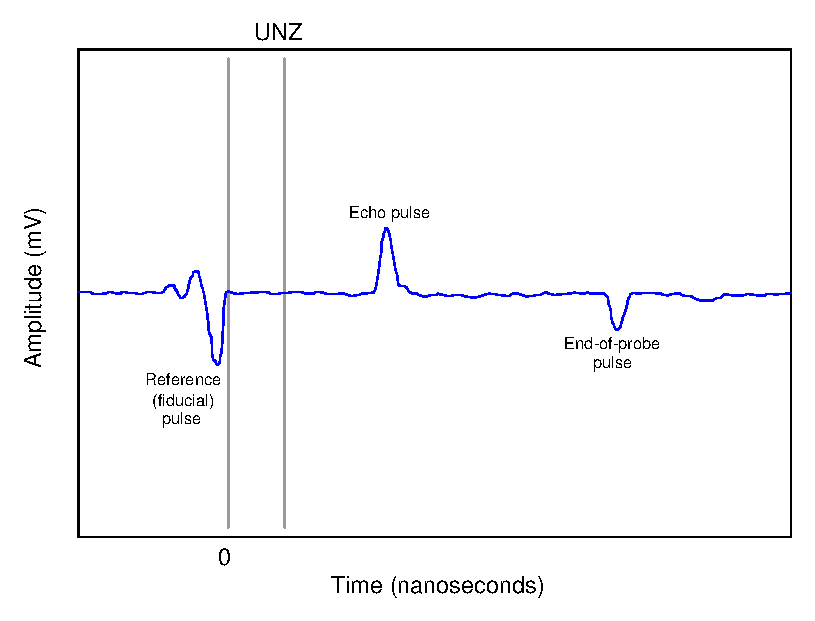
\includegraphics[width=15.5cm]{i00289x01.eps}$$

Forklar hvordan grafen endres hvis:

\begin{itemize}
\item{} Væskenivået øker
\item{} Den dielektriske konstanten ($\epsilon$) til væsken minker
\item{} Tettheten til væsken minker (med konstant $\epsilon$)
\item{} Et væske-væske-grensesnitt med to væsker med ulik tetthet introduseres i tanken
\end{itemize}

Forklar også hva \textit{UNZ} betyr (\textit{Upper Null Zone}).

\vskip 20pt \vbox{\hrule \hbox{\strut \vrule{} {\bf Forslag til sokratisk diskusjon} \vrule} \hrule}

\begin{itemize}
\item{} Beskriv en praktisk grunn til å konfigurere en radartransmitter med upper null zone, og hvordan dette skiller seg fra radarinstrumentets \textit{transition zones}.
\item{} Forklar hvorfor tidsposisjonen til \textit{både} ekkopulsen og end-of-probe-pulsen flytter seg når væskenivået endres i dette systemet.
\end{itemize}

\underbar{file i00289}
%(END_QUESTION)





%(BEGIN_ANSWER)

%(END_ANSWER)





%(BEGIN_NOTES)

Hvis væskenivået øker, vil ekkopulsen komme tidligere (nærmere referansepulsen).

\vskip 10pt

Hvis væskens permittivitet minker, vil end-of-probe-pulsen komme tidligere fordi forplantningshastigheten i væsken øker.  Ekkopulsen blir derimot liggende på samme tid fordi forplantningshastigheten i gassfasen er uendret.  Ekkopulsen blir svakere på grunn av lavere refleksjonsfaktor.

\vskip 10pt

Hvis væskens tetthet minker uten endring i permittivitet, endres ikke ekkotidspunktet i det hele tatt.  Dette viser en viktig fordel ved radarnivåinstrumenter med hensyn til tetthetsendringer.

\vskip 10pt

Hvis et væske-væske-grensesnitt introduseres i tanken, får grafen en ekstra ekkopuls, slik:

$$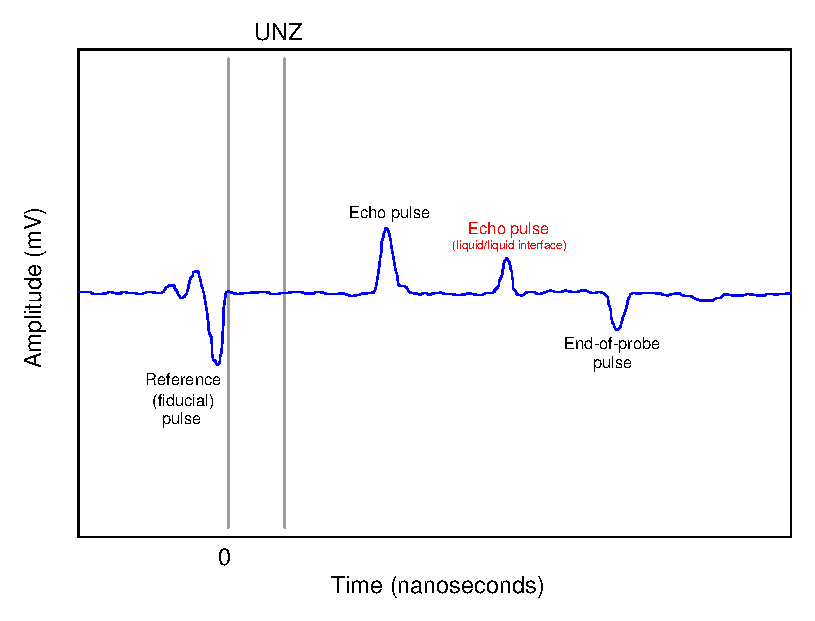
\includegraphics[width=15.5cm]{i00289x03.eps}$$

\vskip 10pt

Upper Null Zone er et område programmert i det digitale radarinstrumentet der reflekterte signaler ignoreres.

\vskip 30pt

\filbreak

Et mer avansert poeng er at når væskenivået øker, flytter ekkopulsen seg nærmere referansepulsen i tid, men end-of-probe-pulsen flytter seg samtidig lenger bort fra referansepulsen, slik:

$$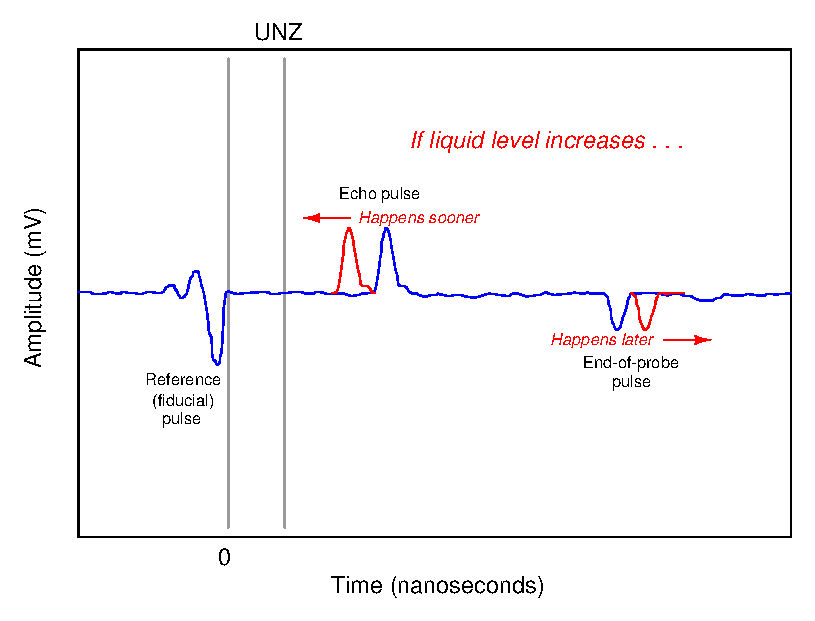
\includegraphics[width=15.5cm]{i00289x02.eps}$$

Grunnen til at end-of-probe-pulsen ikke står fast i tid er at lyshastigheten i væske er lavere enn i damp.  Dette følger naturlig av endringen i permittivitet fra damp til væske:

$$v = {c \over \sqrt{\epsilon_r}}$$

Større væskenivå gir derfor kortere dampvei og dermed kortere tid til ekkopuls.  Samtidig gir det lengre signalvei i væske med lavere forplantningshastighet, slik at retur av end-of-probe-ekko tar lengre tid.

%INDEX% Measurement, level: radar

%(END_NOTES)
